%%
%% This is file `sample-manuscript.tex',
%% generated with the docstrip utility.
%%
%% The original source files were:
%%
%% samples.dtx  (with options: `manuscript')
%% 
%% IMPORTANT NOTICE:
%% 
%% For the copyright see the source file.
%% 
%% Any modified versions of this file must be renamed
%% with new filenames distinct from sample-manuscript.tex.
%% 
%% For distribution of the original source see the terms
%% for copying and modification in the file samples.dtx.
%% 
%% This generated file may be distributed as long as the
%% original source files, as listed above, are part of the
%% same distribution. (The sources need not necessarily be
%% in the same archive or directory.)
%%
%% The first command in your LaTeX source must be the \documentclass command.
%%%% Small single column format, used for CIE, CSUR, DTRAP, JACM, JDIQ, JEA, JERIC, JETC, PACMCGIT, TAAS, TACCESS, TACO, TALG, TALLIP (formerly TALIP), TCPS, TDSCI, TEAC, TECS, TELO, THRI, TIIS, TIOT, TISSEC, TIST, TKDD, TMIS, TOCE, TOCHI, TOCL, TOCS, TOCT, TODAES, TODS, TOIS, TOIT, TOMACS, TOMM (formerly TOMCCAP), TOMPECS, TOMS, TOPC, TOPLAS, TOPS, TOS, TOSEM, TOSN, TQC, TRETS, TSAS, TSC, TSLP, TWEB.
% \documentclass[acmsmall]{acmart}

%%%% Large single column format, used for IMWUT, JOCCH, PACMPL, POMACS, TAP, PACMHCI
% \documentclass[acmlarge,screen]{acmart}

%%%% Large double column format, used for TOG
% \documentclass[acmtog, authorversion]{acmart}

%%%% Generic manuscript mode, required for submission
%%%% and peer review
%\documentclass[manuscript,screen,review]{acmart}
\documentclass[sigconf,screen]{acmart}


%% Fonts used in the template cannot be substituted; margin 
%% adjustments are not allowed.
%%
%% \BibTeX command to typeset BibTeX logo in the docs
\AtBeginDocument{%
 \providecommand\BibTeX{{%
   \normalfont B\kern-0.5em{\scshape i\kern-0.25em b}\kern-0.8em\TeX}}}
    
  %  \AtBeginDocument{\renewcommand*{\thesubfigure}{\alphalph{\value{subfigure}}}}

%% Rights management information.  This information is sent to you
%% when you complete the rights form.  These commands have SAMPLE
%% values in them; it is your responsibility as an author to replace
%% the commands and values with those provided to you when you
%% complete the rights form.


\setcopyright{none} % remove permission section
\settopmatter{printacmref=false, authorsperrow=4} % remove ACM reference format
\renewcommand\footnotetextcopyrightpermission[1]{} % removes footnote with conference information in first column
%\setcopyright{acmcopyright}
%\copyrightyear{2022}
%\acmYear{2022}
%\acmDOI{00.0000/0000000.0000000}


\usepackage{xspace}
\newcommand{\ie}{\textit{i.e.}\xspace}
\newcommand{\eg}{\textit{e.g.}\xspace}
\newcommand{\etal}{\textit{et al.}\xspace}
%\usepackage{array}
%\newcolumntype{L}{>{\arraybackslash}m{8cm}}
%%%%% Long text wrap %%%%%
\usepackage{array}
\newcolumntype{L}{>{\arraybackslash}m{16cm}}
%\newcolumntype{L}[1]{>{\raggedright\let\newline\\arraybackslash\hspace{0pt}}m{#1}}
\newcolumntype{C}[1]{>{\centering\let\newline\\\arraybackslash\hspace{0pt}}m{#1}}
\newcolumntype{R}[1]{>{\raggedleft\let\newline\\\arraybackslash\hspace{0pt}}m{#1}}
%%%%% Long text wrap %%%%%
%\usepackage{adjustbox}
%\usepackage{subcaption}
%\usepackage{textcomp}
%\usepackage{pgfplots}
\usepackage[numbered]{bookmark}
%\usepackage{soul}
%\usepackage{booktabs}
%\usepackage{multirow}
%\usepackage{float}
%\usepackage{url}
\usepackage{tcolorbox}
\usepackage{graphicx}
%\usepackage{textcomp}
\usepackage{xcolor}

%\usepackage{url}
%\usepackage{tabularx} 
%\usepackage{balance}
\usepackage{stfloats}
%\usepackage{fullpage}
\usepackage[justification=centering]{caption}
\usepackage{lineno}
\usepackage[title]{appendix}
\usepackage{dirtytalk}
\usepackage{amsmath}
%\usepackage{tikz}
\usepackage{pgfplots, pgfplotstable}
%\usetikzlibrary{tikzmark}
\usetikzlibrary{patterns}



%%%%%
%-----------------------
%\usepackage[utf8]{inputenc}
\usepackage[english]{babel}
%\usepackage{amssymb}
\usepackage{textcomp}
%\usepackage{indentfirst}
%\setcounter{tocdepth}{3}
\usepackage{mathtools}
%\usepackage[usestackEOL]{stackengine}
%\usepackage{amsmath}
\usepackage{ltxtable}
\usepackage{algorithm}
\usepackage{algpseudocode}
\usepackage{textcomp}
%\usepackage{mathpazo}
%\usepackage{tgpagella}
%-----------------------
\usepackage{enumitem}


%\usepackage[dvipsnames]{xcolor}
\usepackage{pgf-pie}
%\usepackage{pgfplots}
%\pgfplotsset{compat=1.14}
%%%%%%%%%%%%%%%%%%%%%%%%%%%%%%%%%%%%%%%%%%%%%%%%%%%
\definecolor{wedge1}{RGB}{ 190  30  46}
\definecolor{wedge2}{RGB}{ 240  65  54}
\definecolor{wedge3}{RGB}{ 241  90  43}
\definecolor{wedge4}{RGB}{ 247 148  30}
\definecolor{wedge5}{RGB}{  43  56 144}
\definecolor{wedge6}{RGB}{  28 117 188}
\definecolor{wedge7}{RGB}{  40 170 225}
\definecolor{wedge8}{RGB}{ 119 179 225}
\definecolor{wedge9}{RGB}{ 181 212 239}
\definecolor{wedge10}{RGB}{  0 104  56}
\definecolor{wedge11}{RGB}{  0 148  69}
\definecolor{wedge12}{RGB}{ 57 181  74}
\definecolor{wedge13}{RGB}{141 199  63}
\definecolor{wedge14}{RGB}{215 244  34}
\definecolor{wedge15}{RGB}{249 237  50}
\definecolor{wedge16}{RGB}{248 241 148}
\definecolor{wedge17}{RGB}{242 245 205}
\definecolor{wedge18}{RGB}{123  82  49}
\definecolor{wedge19}{RGB}{104  73 158}
\definecolor{wedge20}{RGB}{102  45 145}
\definecolor{wedge21}{RGB}{148 149 151}
\definecolor{wedge22}{RGB}{ 204 50 153}
\definecolor{wedge23}{RGB}{ 79 47 79}
\definecolor{wedge24}{RGB}{ 173 234 234}
\definecolor{wedge25}{RGB}{ 216 191 216}
\definecolor{wedge26}{RGB}{  43  56 144}
\definecolor{wedge27}{RGB}{  40 170 225}
\definecolor{wedge28}{RGB}{ 119 179 225}
\definecolor{wedge29}{RGB}{ 181 212 239}
\definecolor{wedge30}{RGB}{  0 104  56}
\definecolor{wedge31}{RGB}{  0 148  69}
\definecolor{wedge32}{RGB}{ 57 181  74}

\usetikzlibrary{chains}
%%%%%%%%%%%%%%%%%%%%%%%%%%%%%%%%%%%%%%


\def\groupTotals{{1,4,5,8,1,2}}
\pgfmathsetmacro\startAngle{90-3.6/2}
\pgfmathsetmacro\radius{+5}
\pgfmathsetmacro\maxLeg{+12}
\pgfmathsetmacro\legBound{+60}
\pgfmathsetmacro\legSpacing{2*\legBound/(\maxLeg-1)}
%%%%%%%%%%%%%%%%%%%%%%%%%%%%%%%%%%%%%%

%%%%%%%%%%%%%%%%%%%%%%%%%%%%%%%%%%%%%
\usepackage{verbatim}
%\usepackage{pgfplots, pgfplotstable}
%\pgfplotsset{width=7cm,compat=1.8}
%\pgfplotsset{width=7cm,compat=1.8,tick label style={font=\small}}
\pgfplotsset{compat=1.14}
\usetikzlibrary{patterns,}

\usepackage{tabularx,booktabs}
\usepackage{array}
\usepackage{bbding}
\usepackage{pifont}
\usepackage{wasysym}
%\usepackage{amssymb}
\usepackage{caption}
\usepackage{dirtytalk}
%\usepackage[showframe]{geometry}
%\usepackage{subfigure}
\usepackage{subcaption}
%\usepackage{amsmath} % Star
%\usepackage[table]{xcolor}
\usepackage{tabularx}
%\usepackage{pgfplots}
%\usepackage{pgf-pie}
%\usepackage{verbatim}
%\usepackage{pgfplotstable}
\usepackage{sfmath}
\usepackage{array, booktabs, makecell}
\usepackage{color}
%\usepackage[dvipsnames]{xcolor}
\usepackage{csquotes}
\usepackage{url}
\usepackage{comment}
\usepackage{tikz}
\usepackage{balance}
\usepackage{listings}
\usepackage{booktabs} % used for \toprule in tables
%\usepackage{cite}
\usepackage{soul} % highlighting
\urlstyle{same} %% footnote fonts
\usetikzlibrary{fit} %% Used for putting dotted box in image
%\usepackage[margin=2cm]{geometry}
\usetikzlibrary{positioning}
\usetikzlibrary{arrows}
\usetikzlibrary{shapes.multipart}
%\usepackage{caption}
%\usepackage{graphicx}
\usepackage{adjustbox}
%\usepackage{tablefootnote}
\usepackage{float}
\usepackage{rotating}
\usepackage{nth}
\DeclareCaptionType{TextBox}
\usepackage{pstricks}
%%%%%%%%%%%%%%%%%%%%%%%%%%%%%%%%%%%%%%%%%%%%%%%%%%%%%%%%
\usepackage{placeins}
\usepackage{afterpage}
\usepackage{multirow} 
\usepackage{textcomp}
\usepackage{multicol}
\usepackage{varwidth} % Double column tables

%%%%%

%\usepackage{subfigure}
\newcommand{\eman}[1]{\textcolor{violet}{{\it [Eman says: #1]}}}




%%
%% Submission ID.
%% Use this when submitting an article to a sponsored event. You'll
%% receive a unique submission ID from the organizers
%% of the event, and this ID should be used as the parameter to this command.
%%\acmSubmissionID{123-A56-BU3}

%%
%% The majority of ACM publications use numbered citations and
%% references.  The command \citestyle{authoryear} switches to the
%% "author year" style.
%%
%% If you are preparing content for an event
%% sponsored by ACM SIGGRAPH, you must use the "author year" style of
%% citations and references.
%% Uncommenting
%% the next command will enable that style.
%%\citestyle{acmauthoryear}

%%
%% end of the preamble, start of the body of the document source.
\makeatletter
\renewcommand{\thesection}{\arabic{section}}
\renewcommand{\@seccntformat}[1]{\csname the#1\endcsname.\quad}
\makeatother
\begin{document}

\hypersetup{
  colorlinks=true,
  citecolor=blue,
  urlcolor=blue,
  linkcolor=blue
}

%%
%% The "title" command has an optional parameter,
%% allowing the author to define a "short title" to be used in page headers.
\title{Beyond Exact Copies: Detecting Edited Copies of AI Agent Skills}


\author{Bhavesh Maurya}
\email{bmaurya@stevens.edu}
\affiliation{\institution{Stevens Inst. of Tech.}\country{}}

\author{Abhishek Thakkar}
\email{athakkar1@stevens.edu}
\affiliation{\institution{Stevens Inst. of Tech.}\country{}}

\author{Mahima Jain}
\email{mjain19@stevens.edu}
\affiliation{\institution{Stevens Inst. of Tech.}\country{}}

\author{Pratiksha Vilas Pawar}
\email{ppawar6@stevens.edu}
\affiliation{\institution{Stevens Inst. of Tech.}\country{}}
  

%%
%% The "author" command and its associated commands are used to define
%% the authors and their affiliations.
%% Of note is the shared affiliation of the first two authors, and the
%% "authornote" and "authornotemark" commands
%% used to denote shared contribution to the research.


%%
%% By default, the full list of authors will be used in the page
%% headers. Often, this list is too long, and will overlap
%% other information printed in the page headers. This command allows
%% the author to define a more concise list
%% of authors' names for this purpose.
%\renewcommand{\shortauthors}{Trovato and Tobin, et al.}

%%
%% The abstract is a short summary of the work to be presented in the
%% article.

% \begin{abstract}

% Coding agents load agent skills, provided as \texttt{SKILL.md} instruction files, on-demand. The skills are authored by developers, shared across repositories, and regularly modified in the course of re-use. There is no package manager for skills, and thus any modification removes the provenance of a copied skill and makes it impossible to know where it came from. Previous work has tried linking copies based on registry name, fork relation, or exact version. However, similarity-based clone detection alone cannot differentiate an edited copy of a skill from a skill created anew from the same template. \\
% Based on the GitSkills dataset, we manually labeled 100 real pairs of skills as being either derived variants, template siblings, or unrelated. Then we trained a classifier that employs lexical signals combined with features that consider boilerplate and metadata information, as well as structural and repository information. Our classifier achieves an F1 score of 0.98 for identifying derived variants, while the baseline classifier, similar to SkillReuse, reaches only 0.68. When tested on highly similar but not derived pairs, our classifier marks 2\% as derived, while similarity-based baselines label 29-69\% as derived. Importantly, approximately one in five derived pairs of skills has different names and different content hashes, and thus is invisible to approaches based on exact matching and name matching.

% \end{abstract}

\begin{abstract}
Developers reuse agent skills, the \texttt{SKILL.md} instruction files that coding agents load on demand, by copying them between repositories and frequently modifying them in the process. In the absence of a package manager, nothing records where a modified copy came from. Current work on reuse links copies through registry names, forks, or identical versions, while clone detection based on similarity alone cannot distinguish a modified copy from another skill generated from the same template. We annotate 400 real skill pairs from the GitSkills dataset as derived variants, template siblings, or unrelated (Cohen's $\kappa = 0.95$) and train a classifier using lexical, boilerplate-aware, metadata, code, structural, and repository features, with boilerplate lines counted over all 1.59 million in-scope skills of the dataset. It classifies derived variants with an F1 of 0.94 (95\% CI 0.89--0.97), against 0.74 for a SkillReuse-style baseline, and does not classify any of the 159 highly similar non-derived pairs as derived. Applied to 9.0 million candidate pairs, it predicts 4.1 million derivation links; a blinded manual check of 80 randomly drawn links confirms 79 (precision 0.99, 95\% CI 0.93--1.00). Counting reuse by derivation family instead of by exact file hash raises the Gini coefficient of reuse from 0.49 to 0.61--0.63 and the share of files in the top 1\% of units from 27\% to 40--42\%, so reuse is much more concentrated than exact copies suggest.
\end{abstract}


%%
%% Keywords. The author(s) should pick words that accurately describe the work being presented. Separate the keywords with commas.
%\keywords{software quality, mining software repositories}

%% A "teaser" image appears between the author and affiliation information and the body of the document, and typically spans the
%% page.

\begin{teaserfigure}
\vspace{0.3mm}
\end{teaserfigure}

%%
%% This command processes the author and affiliation and title information and builds the first part of the formatted document.
\maketitle
\pagestyle{plain}


% Placeholders for every number the scripts generate. results/macros_*.tex overrides them with \renewcommand. If something still shows in red, the matching script has not been run (or its output was not copied into results/).
\newcommand{\tbd}[1]{\textcolor{red}{\textbf{[#1]}}}
\newcommand{\defres}[1]{\expandafter\newcommand\csname #1\endcsname{\tbd{#1}}}

% 01_extract.py
\defres{ResOccTotal}\defres{ResContentsTotal}\defres{ResReposTotal}\defres{ResOwnersTotal}
\defres{ResWorkContents}\defres{ResWorkOcc}\defres{ResWorkRepos}\defres{ResWorkOwners}
\defres{ResWorkHistory}\defres{ResWorkSiblings}\defres{ResNamesTwoPlus}
\defres{ResFunnelZero}\defres{ResFunnelOne}\defres{ResFunnelTwo}\defres{ResFunnelThree}
\defres{ResFunnelFour}
% 02_candidates.py
\defres{ResCandTotal}\defres{ResCandLSH}\defres{ResCandName}\defres{ResCandLSA}
\defres{ResBandZero}\defres{ResBandOne}\defres{ResBandTwo}\defres{ResBandThree}
\defres{ResBandFour}\defres{ResBandFive}\defres{ResBandSix}
% 03_sample_pairs.py
\defres{ResSampleOne}\defres{ResSampleTwo}\defres{ResSampleThree}\defres{ResSampleFour}
\defres{ResSampleFive}\defres{ResSampleSix}\defres{ResSampleSeven}\defres{ResSampleTotal}
% 04_agreement.py
\defres{ResGoldPairs}\defres{ResGoldDerived}\defres{ResGoldTemplate}\defres{ResGoldUnrelated}
\defres{ResKappaThree}\defres{ResKappaBin}\defres{ResAgree}\defres{ResDisagree}
% 05_features.py
\defres{ResBoilerLines}\defres{ResBoilerK}
% 06_rq1_rq2.py
\defres{ResOursName}\defres{ResOursP}\defres{ResOursR}\defres{ResOursF}\defres{ResOursMCC}
\defres{ResOursHiFP}\defres{ResBaseName}\defres{ResBaseF}\defres{ResBaseHiFP}\defres{ResSRF}
\defres{ResMacroF}\defres{ResTopAblation}\defres{ResTopAblationDrop}\defres{ResGrouping}
% 07_rq3.py
\defres{ResGoldDerivedDiffName}\defres{ResEdgesDiffName}\defres{ResEdgesCrossOwner}
\defres{ResWorkHashes}\defres{ResFamilies}\defres{ResInflation}\defres{ResMultiFamilies}
\defres{ResLargestFamily}\defres{ResLargestCC}\defres{ResDerivedEdges}\defres{ResCandPairs}
\defres{ResGiniHash}\defres{ResGiniFam}\defres{ResCrossHash}\defres{ResCrossFam}\defres{ResOrient}
\defres{ResEmbModel}\defres{ResEmbChunks}\defres{ResEmbWords}
\defres{ResPhaseTwoF}\defres{ResPhaseTwoHiFP}\defres{ResSemanticGain}
\defres{ResOursFLo}\defres{ResOursFHi}\defres{ResBaseFLo}\defres{ResBaseFHi}\defres{ResDiffFLo}\defres{ResDiffFHi}
\defres{ResMcNemarOnlyOurs}\defres{ResMcNemarOnlyBase}\defres{ResMcNemarP}
\defres{ResPhaseTwoFLo}\defres{ResPhaseTwoFHi}\defres{ResPhaseMcNemarOnlyNew}\defres{ResPhaseMcNemarOnlyOld}\defres{ResPhaseMcNemarP}
% full-dataset run
\defres{ResFullOccTotal}\defres{ResFullContentsTotal}\defres{ResFullReposTotal}\defres{ResFullOwnersTotal}
\defres{ResFullWorkContents}\defres{ResFullWorkOcc}\defres{ResFullWorkRepos}\defres{ResFullWorkOwners}
\defres{ResFullWorkHistory}\defres{ResFullWorkSiblings}\defres{ResFullNamesTwoPlus}
\defres{ResFullFunnelZero}\defres{ResFullFunnelOne}\defres{ResFullFunnelTwo}\defres{ResFullFunnelThree}\defres{ResFullFunnelFour}
\defres{ResFullCandTotal}\defres{ResFullCandLSH}\defres{ResFullCandName}\defres{ResFullMaxBucket}\defres{ResFullAnchors}\defres{ResFullBigBuckets}
\defres{ResFullBandZero}\defres{ResFullBandOne}\defres{ResFullBandTwo}\defres{ResFullBandThree}\defres{ResFullBandFour}\defres{ResFullBandFive}
\defres{ResFullBoilerLines}
% provenance
\defres{ResProvAttributionDerived}\defres{ResProvAttributionTemplate}\defres{ResProvAttributionUnrelated}
\defres{ResProvLinkDerived}\defres{ResProvLinkTemplate}\defres{ResProvLinkUnrelated}
\defres{ResProvBundledFileDerived}\defres{ResProvBundledFileTemplate}\defres{ResProvBundledFileUnrelated}
\defres{ResProvHistoryDerived}\defres{ResProvHistoryTemplate}\defres{ResProvHistoryUnrelated}
% validation of predicted links
\defres{ResValPairs}\defres{ResValEdges}\defres{ResValDecoys}\defres{ResValKappa}\defres{ResValAgree}
\defres{ResValPrecision}\defres{ResValPrecLo}\defres{ResValPrecHi}\defres{ResValDecoyDerived}
\defres{ResValConfirmedDiffName}\defres{ResValConfirmedCrossOwner}
\defres{ResValNSameName}\defres{ResValPrecSameName}\defres{ResValPrecSameNameLo}\defres{ResValPrecSameNameHi}
\defres{ResValNDiffName}\defres{ResValPrecDiffName}\defres{ResValPrecDiffNameLo}\defres{ResValPrecDiffNameHi}
\defres{ResValNHiSim}\defres{ResValPrecHiSim}\defres{ResValPrecHiSimLo}\defres{ResValPrecHiSimHi}
\defres{ResValNLowSim}\defres{ResValPrecLowSim}\defres{ResValPrecLowSimLo}\defres{ResValPrecLowSimHi}
% same-name RQ3 variant
\defres{ResSNGoldDerivedDiffName}\defres{ResSNEdgesDiffName}\defres{ResSNEdgesCrossOwner}\defres{ResSNWorkHashes}
\defres{ResSNFamilies}\defres{ResSNInflation}\defres{ResSNMultiFamilies}\defres{ResSNLargestFamily}\defres{ResSNLargestCC}
\defres{ResSNDerivedEdges}\defres{ResSNCandPairs}\defres{ResSNGiniHash}\defres{ResSNGiniFam}\defres{ResSNCrossHash}
\defres{ResSNCrossFam}\defres{ResSNOrient}

% Include a generated table if it exists, otherwise show a red placeholder.
\newcommand{\restable}[2]{\IfFileExists{results/#1}{\input{results/#1}}{\tbd{#2}}}
% Same, but shrinks a generated table to the column width if it is wider (never enlarges).
\newcommand{\restablefit}[2]{\IfFileExists{results/#1}{\adjustbox{max width=\columnwidth}{\input{results/#1}}}{\tbd{#2}}}

\InputIfFileExists{results/macros_extract.tex}{}{}
\InputIfFileExists{results/macros_candidates.tex}{}{}
\InputIfFileExists{results/macros_sample.tex}{}{}
\InputIfFileExists{results/macros_agreement.tex}{}{}
\InputIfFileExists{results/macros_features.tex}{}{}
\InputIfFileExists{results/macros_rq1.tex}{}{}
\InputIfFileExists{results/macros_rq3.tex}{}{}
\InputIfFileExists{results/macros_embeddings.tex}{}{}
\InputIfFileExists{results/macros_stats.tex}{}{}
\InputIfFileExists{results/macros_full_extract.tex}{}{}
\InputIfFileExists{results/macros_full_candidates.tex}{}{}
\InputIfFileExists{results/macros_full_features.tex}{}{}
\InputIfFileExists{results/macros_stats.tex}{}{}
\InputIfFileExists{results/macros_provenance.tex}{}{}
\InputIfFileExists{results/macros_validation.tex}{}{}
\InputIfFileExists{results/macros_rq3_samename.tex}{}{}


\section{Introduction}
\label{Section:Introduction}

Agent-based assistants like Claude Code have been integrated into the daily routine of software developers, who use them to edit files, run commands, and check code changes on their behalf. In order for an agent to do a job as specified by the team's procedure, developers define the procedure as an \emph{agent skill}. A skill is a directory containing a \texttt{SKILL.md} file, which consists of YAML front matter including a \texttt{name} and a \texttt{description}, followed by instructions in Markdown; scripts and reference documents may be included in the directory as well~\cite{agentskills_spec, destefanis2027gitskills}. At first, the agent reads just the descriptions of the skills, and it loads the detailed instructions of a skill only when the task fits its description. The format was introduced as an open standard by Anthropic in October 2025, and just nine months later millions of \texttt{SKILL.md} files were stored in public GitHub repositories~\cite{destefanis2027gitskills}. \\
The libraries included in an application through npm or PyPI are recorded in the manifest file, pinned to a specific version, and installed with the help of the package manager. Skills do not have such an installation procedure. Developers simply copy the directory with the skill into their code base, with any edits performed along the way, without leaving any trace of the origin of the skill. The GitSkills dataset shows how common this is: of the 3,797,117 \texttt{SKILL.md} files found in 282,200 repositories, 50.5\% are exact binary copies of another file in the dataset~\cite{destefanis2027gitskills}. Edited copies are not counted in this statistic, since any edit changes the content hash. \\
The following definitions are used throughout the paper. An \emph{exact copy} has the same content hash as another file. A \emph{derived variant} is a skill created by copying another skill and modifying it through renaming, trimming, extending, rephrasing, or translation; two skills copied from the same source are derived variants of each other. A \emph{template sibling} has only a generic structure in common with another skill, such as section names, general instructions, or the style of a catalog, while the rest of its instructions were written independently. A group of skills connected by derivation forms a \emph{skill family}, and the derivation links within a family form its \emph{lineage}. We call reuse \emph{hidden} when two skills are derived from one another but share neither a content hash nor a front-matter name, so that neither exact matching nor name matching can connect them. These notions are borrowed from clone detection in software engineering, where clones range from exact copies (Type-1) to copies with renamed identifiers (Type-2) and copies with added, removed, or changed statements (Type-3)~\cite{roy2009comparison}. \\
Lineage is important because an agent executes a skill instead of just showing it to a reader. A human who reads an out-of-date README file may notice the issue and work around it, but an agent simply follows the out-of-date instructions of a skill~\cite{gao2026registry}. Skills can even be dangerous. Audits of publicly available skills have found both vulnerable and malicious skills~\cite{liu2026wild}, and in January 2026, one campaign alone introduced more than 1,200 malicious skills to the OpenClaw skill marketplace~\cite{zhu2026skillreuse}. After a flawed skill is copied and altered, finding its descendants becomes difficult. \\
A concrete case from our data shows the problem. One skill in GitSkills is a verbatim copy of a ClickHouse database skill, published under a different name, with an added section that sets up a reverse shell (pair V103 of our validation sample, taken from a benchmark of malicious skills). The two files share neither a content hash nor a name, so neither exact nor name matching can connect the malicious copy to its benign source. Our classifier links them, and both annotators confirmed the link. \\
To address these challenges, we investigate three research questions:\\
{\textbf{RQ1.}} \emph{How accurately does our approach recognise derived skill variants, compared with exact hashing, similarity thresholds, and SkillReuse?}\\
{\textbf{RQ2.}} \emph{Which signals contribute most to separating derived skill variants from template siblings and unrelated skills?}\\
{\textbf{RQ3.}} \emph{How much skill reuse is hidden from exact and name matching, and how does counting it change the picture of reuse?}


\section{Related Work}
\label{Section:RelatedWork}

\subsection{Reuse and adaptation of agent skills}

An early analysis of skills as engineered artifacts is due to Gao et al.~\cite{gao2026registry}. They gathered 18,463 skills from the skills.sh registry and 23,199 skills from 5,876 GitHub repositories. To link a repository skill to a registry skill, they first performed an exact match on the YAML \texttt{name}, then used longest-common-subsequence similarity to pick one of the candidates with the same name, and dropped all pairs with less than 0.1 similarity. This yielded 3,709 reuse links. Their results revealed that reuse is often near-exact: 53\% of the reused skills were never changed once adopted. Of the reused skills that were never changed locally, 40.2\% were taken from a registry whose source later changed, while the copies stayed the same. Yet their method only detects copies whose source is known and available on skills.sh and whose YAML name was not changed. They point out that renamed and modified skills are not detected, and that the whole process assumes that reuse goes from the registry to the repositories. In their dataset, 76\% of the collected repository skills are not linked, and some of them may well be reuse that was not detected. \\
Wu et al.~\cite{wu2026adaptation} investigated how published skills are adapted by examining the public forks of six prominent skill repositories. On the basis of 1,126 adaptation instances, they provide a taxonomy of 46 adaptation patterns organised in 13 families and report that 18.6\% of the adaptations add security-sensitive content to the instructions. They also recommend the development of tools that detect inconsistent adaptations. As their results are derived from the GitHub fork relationship, they only apply to copies made by forking those six repositories; when a skill is pasted into an unrelated repository, no fork relationship is left.

\subsection{Reconstructing how skills spread}

Seddik~\cite{seddik2026constellations} reconstructs the propagation of skills in the same GitSkills release as ours. The study clones the default branch of every repository in the dataset, collects the git history of each \texttt{SKILL.md} file, and constructs a dated, directed copy network of 2,193,119 skill adoptions. A few repositories turn out to be the origin of almost all copies, and GitHub stars do not help to detect them. Copies also rarely stay synchronised with their origins: only 11.1\% of the changes applied to a set of identical copies reach all copies in the set, and only 20.9\% of copies adopt a later edit of their origin. The network is built from exact content. Each unique content corresponds to one skill, and the versions of a skill are connected to each other through the edits recorded by git. In our interpretation of the method, copies edited before their first commit share no version with their origin and are therefore not connected to it; the same applies to renamed and translated copies. The study thus shows where an exact copy came from and whether fixes propagate, but it leaves edited copies untouched.

\subsection{Clone detection for agent skills}

Of all skill reuse detectors, SkillReuse~\cite{zhu2026skillreuse} is the most similar to our work. It encodes the YAML metadata, the prose, and the code of a skill as separate channels, and uses the similarities between these channels, together with a bare TF-IDF similarity and structural features, as input to a logistic regression that reaches an F1 of 0.939 on SkillReuse-Bench, a dataset of 300 labelled skill pairs. When run on 137,470 skills scraped from SkillsMP, it places 66.8\% of skills in at least one clone pair, predominantly across authors. The authors explicitly point out two limitations of clone detection: structural similarity does not necessarily imply derivation, so detected pairs may include convergent development, and a clone relationship does not tell which skill is older. Two properties of the benchmark matter for our purpose. For one thing, half of its 150 positive pairs are synthetic mutations rather than actual modifications. For another, its hard negatives are only same-category pairs whose similarity falls between 0.15 and 0.45, so very similar pairs written independently, like two skills generated from a single template, are not included. The families formed as connected components of the clone graph also form chains, and the largest one includes 61,651 skills. Near-duplicate detection has also reached developer tools: drskill gives an alert when two installed skills exceed a MinHash similarity threshold~\cite{drskill}, and skillvariants groups near-clones of a skill found through GitHub code search~\cite{skillvariants}. Like SkillReuse, both tools find similar skills; neither decides whether one skill was copied from another.

\subsection{Code clones and reuse on GitHub}

Clone detection is an established area of research. Roy et al.~\cite{roy2009comparison} describe the usual types of clones and assess detection methods. SourcererCC performs token-based detection of near-miss clones at scale, for extremely large codebases~\cite{sajnani2016sourcerercc}. Lopes et al.~\cite{lopes2017dejavu} found that file duplication is widespread on GitHub. Clone genealogies were introduced by Kim et al.~\cite{kim2005genealogy}, who track groups of clones across versions and distinguish changes applied consistently to all members of a group from inconsistent ones. These methods rely on lexical and syntactic information, which is reliable for source code. Skills, in contrast, are mostly written in natural language and are often generated from common templates, so surface similarity is a weaker signal of shared origin.

\subsection{Summary}

Table~\ref{tab:related} summarises the approaches. Each earlier approach either needs an exact record that survives copying or measures similarity without deciding origin; ours decides origin from content and validates the decision against human labels.

\begin{table*}[t]
\caption{Summary of related work on tracing the reuse of agent skills.}
\label{tab:related}
\small
\begin{tabular}{>{\raggedright\arraybackslash}p{0.11\textwidth}>{\raggedright\arraybackslash}p{0.17\textwidth}>{\raggedright\arraybackslash}p{0.2\textwidth}>{\raggedright\arraybackslash}p{0.21\textwidth}>{\raggedright\arraybackslash}p{0.21\textwidth}}
\toprule
Study & Data & How reuse is traced & Main finding & What it cannot do \\
\midrule
Gao et al.~\cite{gao2026registry} & 18,463 registry and 23,199 GitHub skills & same YAML name, then text similarity & 3,709 reuse links; 40.2\% of unchanged copies miss later source changes & link renamed or heavily edited copies \\
Wu et al.~\cite{wu2026adaptation} & forks of six popular skill repositories & GitHub fork relation & 46 adaptation patterns; 18.6\% add security-sensitive content & see copies pasted into unrelated repositories \\
Seddik~\cite{seddik2026constellations} & GitSkills release, full git histories & identical versions joined by git edit history & 2,193,119 adoptions; few repositories supply most copies & link copies edited before their first commit, renamed or translated \\
Zhu et al.~\cite{zhu2026skillreuse} & 137,470 marketplace skills; 300 labelled pairs & multi-channel similarity, logistic regression & F1 0.939; 66.8\% of skills in a clone pair & separate copying from shared templates \\
This work & GitSkills release (1.59M skills); 400 + 120 labelled pairs & content classifier with boilerplate-aware features & F1 0.94; 0.99 precision of predicted links; family-level concentration & order derived pairs in time (Phase~4) \\
\bottomrule
\end{tabular}
\end{table*}


\section{Problem Statement}
\label{Section:Problem}

A developer adopts a skill by making a copy of the skill's folder in their own repository. The process of acquiring the skill does not involve any registry entry, manifest, or versioning, hence the adoption goes undocumented. Once the copied folder has been modified, tracing its source becomes a challenge. Three stakeholders bear the brunt of this practice. Adopters do not learn about fixes made to the source of a skill they adopted, while the agents that execute the skill continue to act on old and insecure instructions. A skill's author remains unaware of how far the skill has spread and what has been changed in it. A security reviewer who finds a dangerous skill cannot locate its modified copies. \\
Previous work follows the reuse path through a trace that remains unaltered during copying: the skill name registered in a registry~\cite{gao2026registry}, fork relationships~\cite{wu2026adaptation}, or an identical version shared with the source along with its change history~\cite{seddik2026constellations}. In all cases, the reuse trail breaks when the copy is modified before it is committed, renamed, or translated, because nothing identical is left to identify reuse. Clone detection for skills~\cite{zhu2026skillreuse} does not require any of these traces, but it compares how similar skills are rather than where they came from. It may consider two different skills built from the same template as clones, and its benchmark includes no highly similar skills written independently. \\
This gives rise to two problems. First, to our knowledge, no existing solution distinguishes edited copies from template siblings, which makes it impossible to tell reuse that exact matching cannot detect apart from shared scaffolding. Second, as a result, it is unclear what portion of reuse exact matching cannot detect. The problem also has practical implications: when a reviewer detects a harmful skill, the copy network can list its exact copies~\cite{seddik2026constellations}, but not the edited ones, which may still contain the harmful instructions.


\section{Proposed Solution}
\label{Section:Proposed}

We propose to identify derived variants based on the content of the skills alone, as a way of telling them apart from template siblings and measuring the reuse not captured by exact matching. Our approach has two steps. \\
The first step is a classifier that determines, for a particular pair of skills, whether one skill is a derived variant of the other, a template sibling of the other, or unrelated to it. The challenge is to distinguish between the three. Skills are typically short and often built from the same templates, so two independently written skills can be very similar, while a reworded or translated copy can share little text with its source. There is therefore no clear cut-off point for the degree of similarity, and training the classifier on labels obtained from such a cut-off would only teach it the cut-off point. We therefore developed our ground truth manually: team members independently labelled candidate pairs according to a written rubric, and we measured their agreement. Our sample covers all levels of similarity and deliberately contains highly similar template siblings, which SkillReuse-Bench excludes. In addition to lexical similarity, the classifier uses signals aimed at the template problem, including a similarity computed only over the shared lines that do not recur across many unrelated skills, together with front-matter, structural, and repository features. We compare it with exact hashing, MinHash-based and TF-IDF similarity, and a re-implementation of SkillReuse~\cite{zhu2026skillreuse}. \\
The second step applies the classifier to all candidate pairs of the entire GitSkills release~\cite{gitskills_release}, clusters skills into families, and calculates hidden reuse: what percentage of the derived pairs share neither a content hash nor a name, how many of them connect skills of different owners, and how accounting for them alters the view of how concentrated reuse is. Because these estimates rest on predictions, we check a random sample of predicted links by hand and report each estimate together with the measured precision. \\
This approach avoids the restrictions listed above. It requires no registry record, fork link, or shared version at all. Not needing fork links matters in practice: GitHub code search includes a fork only if it has more stars than the parent repository, so only three repositories in GitSkills are forks~\cite{gitskills_sample}. It distinguishes derivation from templating and validates this distinction on real pairs rather than synthetic mutations. It clusters skills into families with community detection, which limits how far a few bridging links can merge unrelated skills into one big family. Finally, it complements the copy network developed by Seddik~\cite{seddik2026constellations}: that network covers exact copies along with their history, whereas we aim to find the edited copies it cannot connect. Both identify files by their git blob hash, which will allow us to match our links against that network directly in Phase~4.


\section{Dataset Extraction}
\label{sec:dataset}

\paragraph{Source.} The course offers GitSkills in the form of a single SQLite database, \texttt{agent\_skills\_release.db}~\cite{gitskills_release}, containing four tables: \texttt{artifacts}, one entry per file occurrence; \texttt{repos}, repository metadata; \texttt{artifact\_\allowbreak siblings}, files bundled with each skill; and the \texttt{mining\_runs}, metadata of data collection~\cite{destefanis2027gitskills}. We rely on it on two levels. The \emph{full release} (\ResFullOccTotal{} file occurrences of \ResFullContentsTotal{} distinct contents in \ResFullReposTotal{} repositories owned by \ResFullOwnersTotal{} accounts) serves as the population of all analyses. The \emph{official sample} was trimmed down from the release by the authors of the dataset~\cite{gitskills_sample}: it contains the \ResContentsTotal{} distinct contents with the smallest content hashes, along with all rows related to them in the release, and it is the source of the pairs we labelled. The content hashes are effectively uniform, so the sample is a random sample of distinct skills; it is structured just like the release, and every labelled pair also occurs in the release.

\paragraph{Fields.} Table~\ref{tab:fields} lists the fields we extract.

\begin{table}[t]
\caption{GitSkills fields used in this study.}
\label{tab:fields}
\small
\begin{tabular}{>{\raggedright\arraybackslash}p{0.55\columnwidth}>{\raggedright\arraybackslash}p{0.35\columnwidth}}
\toprule
Field(s) & Use \\
\midrule
\texttt{file\_sha}, \texttt{repo\_full\_name}, \texttt{path}, \texttt{location\_class} & occurrences, exact-copy counts \\
\texttt{filename}, \texttt{dedup\_primary}, \texttt{frontmatter\_valid}, \texttt{body\_chars} & scope filtering \\
\texttt{content}, \texttt{name}, \texttt{description} & skill text (representatives) \\
\texttt{first\_commit\_at} & history coverage \\
\texttt{artifact\_siblings.entry\_name} & bundled-file similarity \\
owner (prefix of \texttt{repo\_full\_name}) & same-owner and cross-owner reuse \\
\bottomrule
\end{tabular}
\end{table}

\paragraph{Scope.} Since the filename search used by GitSkills catches lowercase \texttt{skill.md} files as well as older files with similar names that predate the format, we retain only representatives whose basename is exactly \texttt{SKILL.md}. We also need valid front matter, since the name and description are used as inputs for our classifier, and a body of at least 200 characters, which filters out stub skills and skills stored as symbolic links (their bodies contain only a link target). Table~\ref{tab:funnel} shows the effect of filtering on both levels; the ratio of contents that pass all filters is the same (85\%), which is expected for a uniform sample.


\begin{table}[t]
\caption{Scope filters applied to the official sample and to the full release.}
\label{tab:funnel}
\small
\begin{tabular}{lrr}
\toprule
Filter & Sample & Full release \\
\midrule
All distinct contents & \ResFunnelZero & \ResFullFunnelZero \\
Exact basename \texttt{SKILL.md} & \ResFunnelOne & \ResFullFunnelOne \\
Valid YAML front matter & \ResFunnelTwo & \ResFullFunnelTwo \\
Body $\geq$ 200 characters (dataset field) & \ResFunnelThree & \ResFullFunnelThree \\
Body $\geq$ 200 characters after our own parsing & \ResFunnelFour & \ResFullFunnelFour \\
\bottomrule
\end{tabular}
\end{table}

The working set of the full release includes \ResFullWorkContents{} skills, which are found in \ResFullWorkOcc{} files in \ResFullWorkRepos{} repositories owned by \ResFullWorkOwners{} accounts. For \ResFullWorkHistory{} of these skills, commit history is available, \ResFullWorkSiblings{} bundle at least one other file, and \ResFullNamesTwoPlus{} front-matter names are used by two or more distinct contents. The working set of the sample includes \ResWorkContents{} skills.

\paragraph{Decomposition.} Each representative file is decomposed into its normalised name, description, prose (body without fenced code blocks), code blocks, and headings. Additionally, we extract the repository context of each skill: the owner accounts of all of its occurrences, the name of the folder the skill is located in, and the names of the bundled files. At this stage we produce a new SQLite database with two tables, \texttt{skills} and \texttt{occurrences} (\texttt{extracted.db} for the sample, \texttt{full\_skills.db} for the full release), which is the input of the following steps.



\section{Study Design}
\label{sec:design}

Figure~\ref{fig:overview} gives an overview of our approach. It has five stages: the first two are automatic, the third is our manual analysis of the dataset, and the last two build the classifier and apply it.

\paragraph{Changes since Phase 2.} Phase 3 extends the study in six ways, each answering a limitation of Phase 2. (i) The gold set doubles from 200 to \ResGoldPairs{} labelled pairs. (ii) Every analysis now runs on the full GitSkills release instead of the official sample. (iii) A blinded manual check measures the precision of the predicted links, so RQ3 is reported conditional on measured precision. (iv) A provenance check tests the labels against evidence that does not come from text similarity (Section~\ref{sec:labelvalidity}). (v) The pipeline is made reproducible: package versions are pinned, the candidate pairs and the labelled sample are stored by content hash, threshold tuning no longer depends on floating-point details of a machine, fenced code is parsed as in CommonMark, and the labelling viewer is published with complete, untruncated skills. (vi) We report confidence intervals and significance tests, and we tried multilingual sentence embeddings to recover translated copies; they did not help (Section~\ref{sec:rq2}).

\begin{figure*}[t]
  \centering
  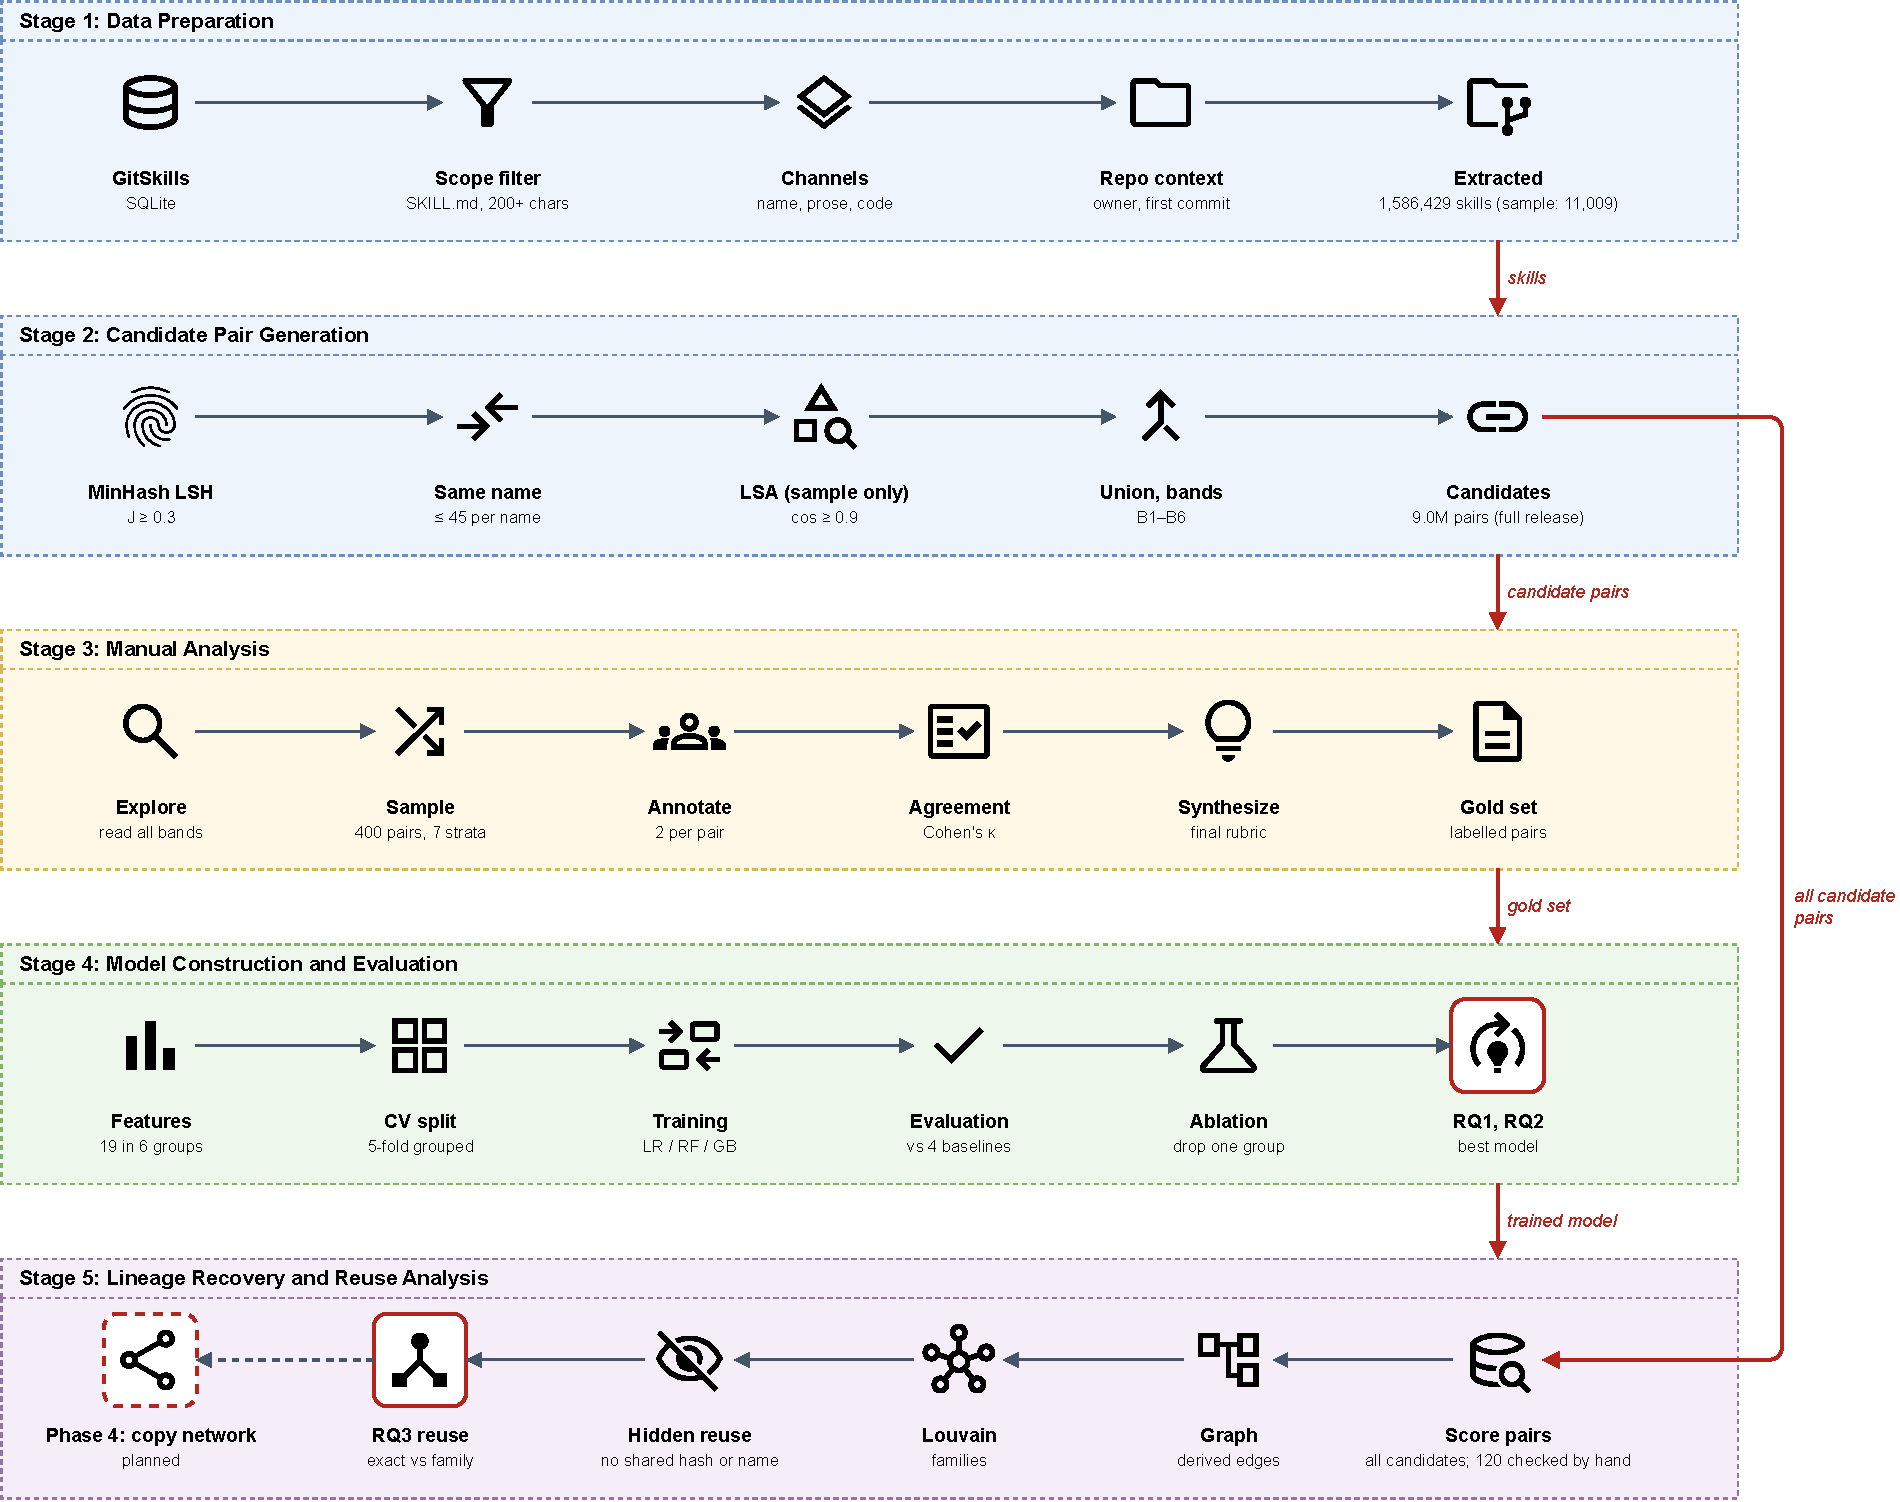
\includegraphics[width=\textwidth]{Images/approach_diagram.pdf}
  \caption{Approach overview. The shaded third stage is manual; outlined boxes answer our research questions, and the dashed box is planned for Phase~4. Stage~5 runs right to left, starting from the trained model and the full set of candidate pairs. The LSA blocker of Stage~2 is used on the official sample only.}
  \label{fig:overview}
\end{figure*}

\paragraph{Stage 1: Data preparation.} We extract the working set described in Section~\ref{sec:dataset} and split each skill into its name, description, prose, code blocks, and headings, together with its repository context.

\paragraph{Stage 2: Candidate pair generation.} Comparing every pair of the \ResFullWorkContents{} skills would take more than a trillion comparisons, so we score only pairs proposed by inexpensive blockers. MinHash locality-sensitive hashing~\cite{broder1997resemblance} over word 5-gram shingles of the body (128 permutations, 37 bands of 3 rows) proposes pairs whose estimated Jaccard similarity is around 0.3 or more, and same-name blocking proposes distinct contents that carry the same normalised front-matter name, capped at 45 pairs per name. On the sample we also used nearest neighbours in a latent semantic analysis (LSA) space~\cite{deerwester1990lsa} to catch reworded copies; in the labelled pairs, the pairs found only by LSA (band B6) contain no derived pair, so we drop this blocker at full scale. Large catalogs of near-identical skills fill single MinHash buckets with thousands of members; we pair each member of a bucket with more than \ResFullMaxBucket{} members with its \ResFullAnchors{} lowest-id members instead of with all of them, which keeps the bucket connected while the number of pairs stays linear (\ResFullBigBuckets{} buckets were capped). On the full release the blockers propose \ResFullCandTotal{} candidate pairs (Table~\ref{tab:bands} gives the bands of the sample, from which the labelled pairs were drawn).

\begin{table}[t]
\caption{Similarity bands of the candidate pairs of the official sample and of the pairs drawn from them for labelling.}
\label{tab:bands}
\small
\begin{tabular}{llrr}
\toprule
Band & Definition & Candidates & Sampled \\
\midrule
B1 & $J \geq 0.9$ & \ResBandOne & \ResSampleOne \\
B2 & $0.7 \leq J < 0.9$ & \ResBandTwo & \ResSampleTwo \\
B3 & $0.5 \leq J < 0.7$ & \ResBandThree & \ResSampleThree \\
B4 & $0.3 \leq J < 0.5$ & \ResBandFour & \ResSampleFour \\
B5 & same name, $J < 0.3$ & \ResBandFive & \ResSampleFive \\
B6 & LSA neighbour, $J < 0.3$ & \ResBandSix & \ResSampleSix \\
B7 & random pair (not a candidate) & -- & \ResSampleSeven \\
B0 & other LSH match, $J < 0.3$ & \ResBandZero & 0 \\
\midrule
 & Total & \ResCandTotal & \ResSampleTotal \\
\bottomrule
\end{tabular}
\end{table}

\paragraph{Stage 3: Manual analysis.} We followed three steps, explore, analyse, and synthesise, and added a fourth in Phase~3, validate.

\emph{Explore.} Before labelling, we inspected candidate skill pairs from all bands using a side-by-side diff view in two columns, plus selected skills, to understand why certain skills look similar to one another. Much of the similarity in the middle bands was due to boilerplate, not copy-and-paste. We discovered a set of machine-generated skills with names \texttt{u02156-...}, which varied only by several words, skills wrapping Rube MCP (Composio) boilerplate for different applications, as well as a set of German legal practice skills containing identical checklist-like lines. However, we also saw a number of pairs with the same name and topic (like two refactoring skills), which were authored independently. These observations led to our three-class labelling scheme.

\emph{Analyse.} The stratified sample included \ResSampleTotal{} pairs from all bands of Table~\ref{tab:bands}, among them \ResSampleSeven{} randomly selected pairs that no blocker had proposed, which serve as easy negatives. For the diversity of the sample, a single skill occurs in at most two candidate pairs and the same name in at most four pairs; the random pairs were drawn without the skill limit, so one skill occurs in a third pair (P0044, P0145 and the random pair P0096). The order of skills in each pair was randomised, and similarity bands and scores were not shown to the annotators, so that neither could bias their labels. Pair identifiers were assigned after randomisation, thus the first 200 pairs, which we annotated in Phase~2, represent a random subset of the sample; Phase~3 included annotation of the other 200 pairs, resulting in \ResGoldPairs{} annotated pairs in total. Two team members independently annotated each pair by criteria we adapted from the ones Gao et al.\ used for validating their reuse links~\cite{gao2026registry}. A pair was considered derived if the skills share distinctive content that is unlikely to be created independently (identical or slightly modified text, as well as task-specific steps, examples, commands, paths, and configuration values; renaming and translation do not change the label). If the only shared parts were scaffolding text, a pair was considered a template sibling pair; otherwise it was an unrelated pair. A shared topic alone cannot be counted as derivation. The annotators agreed on 388 out of \ResGoldPairs{} pairs, obtaining a Cohen's $\kappa$~\cite{cohen1960kappa} of \ResKappaThree{} for the three-class annotations and \ResKappaBin{} for the binary ones (i.e., derived vs.\ not derived). The \ResDisagree{} disagreements were resolved by discussing the examples; all of them were borderline cases, such as a skill that reworks another one's steps without copying any line (P0121), or a pair of skills that share a generated section schema but no actual content (P0185).\footnote{The labelling sheets and the gold set are part of our replication package: \url{https://github.com/BhaveshMRA/RWPM}.}

\emph{Synthesise.} Based on the notes taken during labelling, we grouped the reasons why two skills resemble each other. Derived pairs arise from copy-and-edit, in which a copy is shortened or lengthened (P0000, P0046), from renamed copies (P0022, P0054, P0087), from translated copies (P0137), and from copies whose paths an installer rewrote for another agent tool (P0060, P0092). Template pairs result from catalog generators that only fill slots (P0002, P0008), integration catalogs wrapping many applications in the same manner (P0016, P0028), domain series by the same author (P0036, P0068), and long project preambles shared by several skills (P0003, P0058). Unrelated pairs often share a name or a topic but no text (P0038, P0084). Resolving the disagreements fixed three rules: a standardised structure of the domain, e.g.\ the sections of an architecture decision record, does not make two skills template siblings (P0142); a shared generated skeleton makes them template siblings even without shared content (P0185); and a skill that uses distinctive steps of another skill is derived even when no line is copied verbatim (P0121), as is an installer copy with rewritten paths (P0169). Out of the 75 pairs that at least one of us marked as uncertain, 24 belong to band B5, where two skills have the same name but little text, and 31 connect two skills from the same owner. As a result, the gold set includes \ResGoldPairs{} pairs: \ResGoldDerived{} derived, \ResGoldTemplate{} template, and \ResGoldUnrelated{} unrelated.

\emph{Validate.} Labels on a sample stratified by similarity allow us to assess how well the classifier separates the classes, but not how precise its predictions are on the population. Thus, after applying the classifier to the full release, we selected \ResValEdges{} predicted derivation links at random, together with \ResValDecoys{} random candidate pairs that the classifier predicted as not derived, shuffled them, and labelled all \ResValPairs{} pairs according to the same rubric and viewer, two annotators for each pair. The annotators were unaware of the predictions of the classifier, and they reached complete agreement on all the pairs ($\kappa = $ \ResValKappa{}). We attribute this to the chosen pairs, which are dominated by near-identical copies and catalog templates, whereas the gold set intentionally oversamples the more difficult bands.

\paragraph{Stage 4: Model construction and evaluation.} For each pair we calculate 19 features belonging to six feature groups (Table~\ref{tab:features}). The corpus statistics come from the full release: a normalised line is considered to be \emph{boilerplate} if it occurs in skills with at least \ResBoilerK{} distinct front-matter names, resulting in \ResFullBoilerLines{} boilerplate lines (\ResBoilerLines{} within the sample only); the TF-IDF, LSA and normalisation models are trained just once, on a sample of approximately 50,600 skills of the release (50,000 randomly selected skills and all skills of the gold set), which keeps memory use manageable. Then logistic regression, random forest and gradient boosting classifiers are trained with balanced class weights and evaluated using five-fold stratified group cross-validation, so that no skill is present in both a training and a test fold (Section~\ref{sec:setup}). Section~\ref{sec:whitebox} opens this stage in detail.


\paragraph{Stage 5: Lineage recovery and reuse analysis.} The best classifier from Stage~4 is re-trained on all gold pairs and used to predict the relation of all candidate pairs in the full release. Pairs predicted as derived form the edges of a derivation graph, on which Louvain community detection~\cite{blondel2008louvain} is performed to produce skill families. Since a few false edges may group many skills together, we construct families in two ways: from all predicted edges, and, as a more conservative variant, only from edges between skills with the same front-matter name, which renamed copies cannot enter. We then measure hidden reuse and compare reuse counted by exact hash with reuse counted by family (RQ3). As a check on the labels themselves, we also collect, for each labelled pair, evidence that does not come from text similarity: explicit attribution to a source, shared non-generic bundled files, and whether both skills have a recorded first commit.

\paragraph{Reproducibility.} Package versions are pinned (\texttt{requirements-\allowbreak{}full.txt}, with the entire environment of both machines in the \texttt{requirements-\allowbreak{}lock.txt} and \texttt{requirements-\allowbreak{}mac.txt}). The candidate pairs of the sample are locked in a file that uses content hashes as keys, and the labelled sample is locked the same way, so rerunning the pipeline cannot alter either. Threshold tuning rounds the scores before selecting a threshold, so floating-point differences between machines no longer change baseline decisions. Fenced code blocks are parsed according to the CommonMark rules, and the labelling viewer, which now displays complete, untruncated skills, is published with the labels in the repository. The full-release run streams the database in chunks; run on the official sample, it reproduces the features of the sample pipeline exactly.


\begin{table}[t]
\caption{Pair features used by our classifier.}
\label{tab:features}
\small
\begin{tabular}{>{\raggedright\arraybackslash}p{0.22\columnwidth}>{\raggedright\arraybackslash}p{0.70\columnwidth}}
\toprule
Group & Features \\
\midrule
Lexical & Jaccard and containment of word 5-gram shingles; TF-IDF cosine of the bodies; normalised edit similarity of the first 5,000 characters \\
Boilerplate-aware & Jaccard and containment of distinctive lines; Jaccard of boilerplate lines; share of shared lines that are boilerplate \\
Metadata & names equal; name similarity; TF-IDF cosine of the descriptions \\
Code & Jaccard of identifier tokens in code blocks; both skills contain code \\
Structure & similarity of heading sequences; length ratio; heading-count ratio \\
Repository & a shared owner; same skill-folder name; Jaccard of bundled file names \\
\bottomrule
\end{tabular}
\end{table}

\subsection{White-Box View of the Classifier}
\label{sec:whitebox}

Figure~\ref{fig:overview} shows the classifier only as the Training box of Stage~4. Figure~\ref{fig:whitebox} opens it and follows one candidate pair from its two \texttt{SKILL.md} files to the decision.

\begin{figure*}[t]
  \centering
  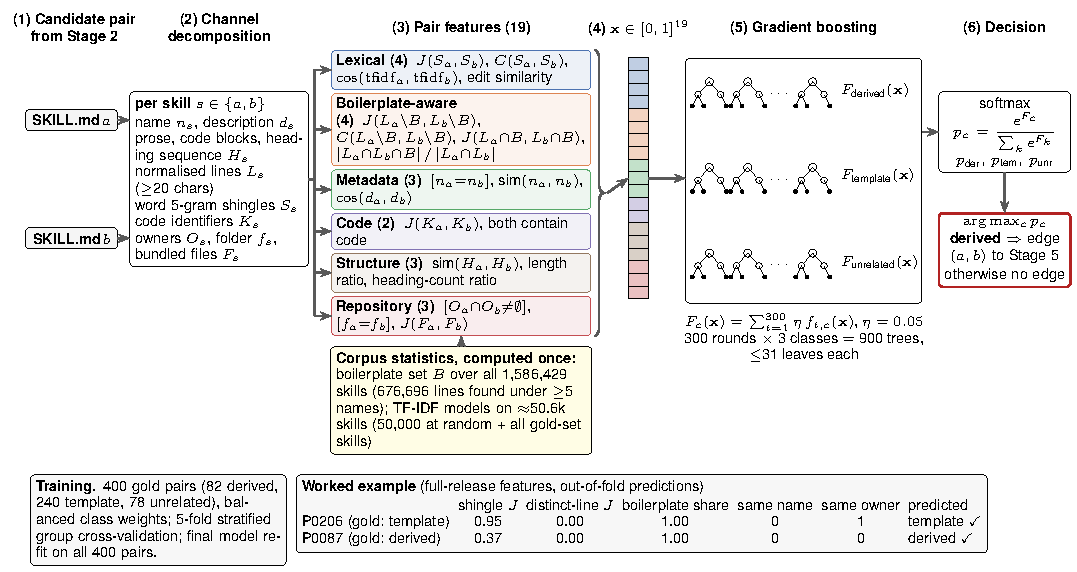
\includegraphics[width=\textwidth]{Images/white_box_model.pdf}
  \caption{White-box view of the classifier (Stage~4 of Figure~\ref{fig:overview}): how a candidate
  pair is decomposed into channels, turned into 19 features in six groups, and classified by
  gradient boosting; derived pairs become edges for Stage~5.}
  \label{fig:whitebox}
\end{figure*}

\emph{(1) Input.} A candidate pair $(a,b)$ proposed by the blockers of Stage~2.

\emph{(2) Channel decomposition.} Each file is split into its front-matter name $n_s$ and description $d_s$, and its body into prose, code blocks and the sequence of headings $H_s$. From the body we derive the set of normalised lines $L_s$ (lower case, list markers removed, whitespace collapsed, at least 20 characters containing a letter), the set of word 5-gram shingles $S_s$, and the set of identifiers $K_s$ in code blocks (split at camel case and underscores). Repository context adds the owners $O_s$ of all copies, the name of the skill's folder $f_s$, and the names of its bundled files $F_s$.

\emph{(3) Pair features.} The two skills are compared channel by channel. Most features are a Jaccard similarity $J(X,Y)=|X\cap Y|/|X\cup Y|$, a containment $C(X,Y)=|X\cap Y|/\min(|X|,|Y|)$, a cosine of TF-IDF vectors, or an equality test. The boilerplate-aware group first removes the lines that belong to the boilerplate set $B$, so that $J(L_a\setminus B, L_b\setminus B)$ measures shared distinctive lines, and adds the share of shared lines that are boilerplate. Neither is computed per pair: $B$ is counted once over all 1,586,429 skills of the release, the TF-IDF models are fitted once on about 50,600 of them, and both are reused for every pair.

\emph{(4) Feature vector.} The 19 values form a vector $\mathbf{x}\in[0,1]^{19}$; every feature is a similarity, a ratio or a binary indicator.

\emph{(5) Gradient boosting.} The classifier runs 300 boosting rounds. In each round it fits one regression tree per class (at most 31 leaves, at least 20 training pairs per leaf, features binned into at most 255 values) to the gradient of the multinomial loss, so the model consists of 900 trees. The score of class $c$ is $F_c(\mathbf{x})=\sum_{t=1}^{300}\eta\,f_{t,c}(\mathbf{x})$ with learning rate $\eta=0.05$, and training weights each class inversely to its frequency, so that 82 derived pairs weigh as much as 240 template pairs.

\emph{(6) Decision.} A softmax turns the three scores into probabilities, and the most probable class is the prediction. A pair predicted as derived becomes an edge of the derivation graph of Stage~5; template and unrelated pairs add no edge.

\emph{Worked example.} The bottom of Figure~\ref{fig:whitebox} shows two labelled pairs. At full scale neither shares a distinctive line: the lines of both pairs occur under five or more names, so all their shared lines are boilerplate. The boilerplate-aware features therefore cannot separate them, and plain similarity would rank them the wrong way round, since the template pair P0206 shares far more text (shingle Jaccard 0.95) than the derived pair P0087 (0.37). The model still classifies both correctly by combining the other groups; for example, the two skills of P0206 belong to one owner, which in the linear view of Figure~\ref{fig:model} is the strongest single indicator of a template.


\section{Experiments}
\label{sec:experiments}

\subsection{Research Questions}

Three research questions assess our solution.

\paragraph{RQ1 (Effectiveness).} \emph{How accurately does our approach recognise derived skill variants, compared with exact hashing, similarity thresholds, and SkillReuse?} This question tests whether derivation can be recognised from content alone, and how our design performs on the pairs that matter most: highly similar pairs that are not derived. We report precision, recall, F1, and the Matthews correlation coefficient (MCC)~\cite{chicco2020mcc} for the \emph{derived} class, computed on pooled out-of-fold predictions, together with the standard deviation of F1 across folds and 95\% bootstrap confidence intervals. We also report the false-positive rate on high-similarity pairs (non-derived pairs in bands B1--B3), precision and recall per band, and, for our approach, a three-class confusion matrix and macro-F1.

\paragraph{RQ2 (Contributing signals).} \emph{Which signals contribute most to separating derived skill variants from template siblings and unrelated skills?} We remove one feature group at a time, retrain the best model, and measure the change in F1 and in the high-similarity false-positive rate. We also train a model on lexical features alone.

\paragraph{RQ3 (Hidden reuse).} \emph{How much skill reuse is hidden from exact and name matching, and how does counting it change the picture of reuse?} This question measures what hash-, name-, and version-based approaches leave out. Among the labelled derived pairs, we measure the share whose front-matter names differ; since the two skills of every pair also have different content hashes, these pairs are invisible to both exact and name matching. Among all derivations predicted by the best model, we measure the share with different names and the share that crosses owners. We then compare two units of reuse, exact hash and derivation family, by the number of units, the inflation ratio (distinct contents per family), the size of the largest family, the Gini coefficient of file occurrences per unit, and the share of units spanning two or more owners. We leave the comparison with the copy network of Seddik~\cite{seddik2026constellations} to Phase~4.

\subsection{Experimental Setup}
\label{sec:setup}

RQ1 and RQ2 use the \ResGoldPairs{} gold pairs; RQ3 uses the predictions on the full release and the manually checked sample of them. We use five-fold stratified group cross-validation; groups are formed by \ResGrouping{}, so no skill contributes to both training and testing. We compare four baselines with our approach. \\
\emph{Normalised-text hash} predicts \emph{derived} only when the two bodies are identical after lower-casing and collapsing whitespace, which is what exact hashing sees once trivial formatting is ignored. \emph{Shingle Jaccard (MinHash)} thresholds the exact Jaccard similarity of word 5-gram shingles, the quantity MinHash estimates. \emph{TF-IDF cosine} thresholds the cosine similarity of TF-IDF vectors of the bodies. For both, the threshold that maximises F1 is chosen on the training folds only. \emph{SkillReuse-style} is our re-implementation of the eight features of Zhu et al.~\cite{zhu2026skillreuse}: a flat TF-IDF similarity, LSA cosine similarities for the YAML, prose, and code channels (set to zero when a channel is missing), their three pairwise products, and a structural similarity over eight document statistics, combined by a class-balanced logistic regression whose threshold is again tuned on the training folds. It is trained on our gold set, so it is compared with our approach on equal terms; it is not the authors' released implementation.

Our approach uses the 19 features of Table~\ref{tab:features} with three classifiers from scikit-learn: logistic regression on standardised features, a random forest with 500 trees, and histogram-based gradient boosting, all with balanced class weights and no threshold tuning. The classifiers are trained on the three classes when the gold set has at least 15 template pairs, and on derived versus not derived otherwise. We report 95\% bootstrap confidence intervals (2,000 resamples of the labelled pairs) and compare our best model with the strongest baseline using McNemar's exact test. On the sample we also tried adding multilingual sentence embeddings (\ResEmbModel{}) as a sixth feature group, aimed at translated and reworded copies (Section~\ref{sec:rq2}).

\subsection{RQ1: Effectiveness}
\label{sec:rq1}

\begin{table*}[t]
\caption{RQ1: detection of derived variants (pooled out-of-fold predictions; F1 $\pm$
standard deviation across folds). The last column is the share of non-derived pairs in bands
B1--B3 that a method labels as derived (lower is better).}
\label{tab:rq1}
\small
\restable{rq1_main.tex}{Run code/06\_rq1\_rq2.py to generate this table.}
\end{table*}

\begin{table*}[t]
\caption{RQ1 by similarity band: precision (P) and recall (R) of the strongest baseline and
of our best model.}
\label{tab:rq1bands}
\small
\restable{rq1_bands.tex}{Run code/06\_rq1\_rq2.py to generate this table.}
\end{table*}

\begin{table}[t]
\caption{RQ1: confusion matrix of our best model (out-of-fold).}
\label{tab:confusion}
\small
\restable{rq1_confusion.tex}{Run code/06\_rq1\_rq2.py to generate this table.}
\end{table}

Table~\ref{tab:rq1} compares all methods. The best configuration of our approach, \ResOursName{}, reaches a precision of \ResOursP{}, a recall of \ResOursR{}, and an F1 of \ResOursF{} (95\% CI \ResOursFLo--\ResOursFHi; MCC \ResOursMCC{}); random forest is almost as good (F1 0.94), while logistic regression drops to 0.87 with full-corpus features, presumably because some feature distributions become very skewed. The strongest baseline, the SkillReuse-style detector, reaches an F1 of \ResBaseF{} (\ResBaseFLo--\ResBaseFHi). The difference in F1 is \ResDiffFLo-\ResDiffFHi{} (95\% CI), and the two methods disagree in a way that is very unlikely by chance: ours is right on \ResMcNemarOnlyOurs{} pairs that the baseline gets wrong, the baseline on \ResMcNemarOnlyBase{} (McNemar's test, $p$ \ResMcNemarP{}). Among the 159 highly similar pairs that annotators judged not derived, our approach labels none as derived, the SkillReuse-style detector 10\%, and MinHash similarity 33\%. Across the three classes our approach reaches a macro-F1 of \ResMacroF{} (Table~\ref{tab:confusion}).

The confusion matrix (Table~\ref{tab:confusion}) shows where the model succeeds and where it fails. It recognises template siblings almost perfectly: 238 of the 240 template pairs are classified correctly and none is called derived, so the confusion behind most baseline false positives does not occur. This is where the design pays off: a template pair shares mostly boilerplate and, typically, an owner, while its names and descriptions differ in the substituted slots. The errors lie elsewhere: eight derived pairs are missed (four called template, four unrelated), two unrelated pairs are called derived, and two template and two unrelated pairs are confused with each other, which affects no derivation link.

Of the 96 false positives of the three similarity baselines, 90 are template pairs, and of the 19 derived pairs that all three miss, our approach finds 13; examples are P0054, which renames the grill-me skill and rewrites its rules around one copied sentence, and P0169, an installer copy of the gsd-manager skill whose paths were rewritten. On the derived class our model makes ten errors (eight missed copies and two false alarms), in three groups. First, four copies share no text with their source: P0121 reworks another skill's steps, P0137 and P0268 are Chinese adaptations, and P0335 keeps only the description; with no shared text, the model calls them unrelated. Second, four copies of two very popular skills, Matt Pocock's improve-codebase-architecture (P0053, P0123, P0297) and Superpowers' verification-before-completion (P0348), three of them renamed, are called templates: at full scale their lines occur under five or more names and therefore count as boilerplate. Third, the two false positives, P0226 and P0270, are unrelated skills that share a name and a topic.

\begin{quote}
\textbf{Answer to RQ1:} Our approach identifies derived variants with an F1 of \ResOursF{} (\ResOursFLo-\ResOursFHi), significantly better than the strongest baseline (\ResBaseF{}), and labels no highly similar non-derived pair as derived. Its errors are copies without shared text, copies of very popular skills, and same-name skills on the same topic.
\end{quote}

\subsection{RQ2: Contributing Signals}
\label{sec:rq2}

\begin{table}[t]
\caption{RQ2: ablation of feature groups for our best model.}
\label{tab:rq2}
\small
\restablefit{rq2_ablation.tex}{Run code/06\_rq1\_rq2.py to generate this table.}
\end{table}

Table~\ref{tab:rq2} reports the ablation. Lexical similarity alone is far from enough: a lexical-only model drops to an F1 of 0.59 and labels a quarter of the highly similar non-derived pairs as derived. No single other group is indispensable; removing any one costs between 0.02 and 0.05 in F1, most for metadata (\ResTopAblationDrop{}). Figure~\ref{fig:model} shows what the best model relies on. On held-out folds, shuffling the metadata features costs most (0.33 in F1), followed by lexical (0.21), repository (0.08) and code (0.07) features; boilerplate-aware features cost only 0.05. On the sample alone, boilerplate-aware features had been the most important group (0.39). With boilerplate counted over the full release, the lines of popular skills that are copied under many names become boilerplate too, so these features separate templates from copies less sharply and the model leans on names and descriptions instead. Adding multilingual sentence embeddings did not help: on the sample, F1 changed from 0.944 to 0.938 (McNemar's test, $p = 1.0$), the embeddings fixed two pairs and broke three, and the translated copies they were meant to catch stayed undetected, because embedding similarity measures topic as much as origin.

\begin{figure}[t]
  \centering
  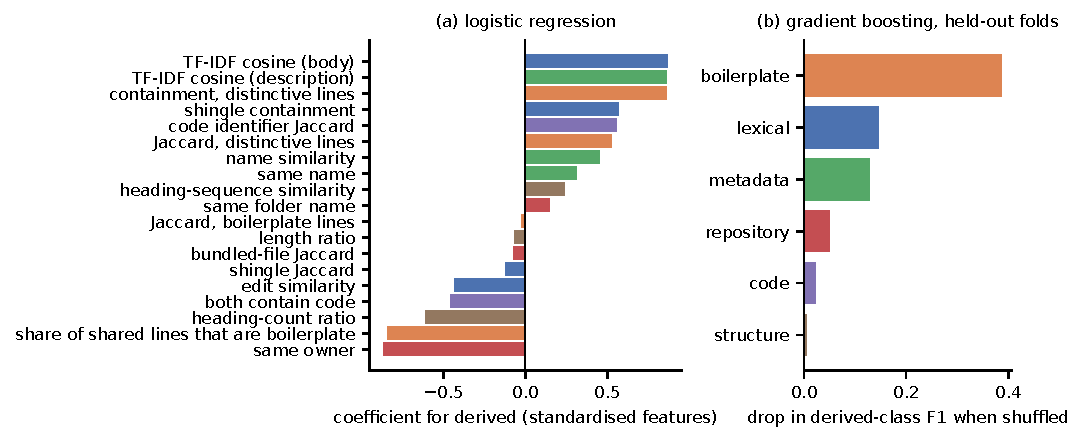
\includegraphics[width=\columnwidth]{results/fig_model.pdf}
  \caption{What the trained model relies on (complementing the white-box view of
  Figure~\ref{fig:whitebox}): (a) logistic-regression coefficients for the derived class on
  standardised features; (b) drop in derived-class F1 of the best model on held-out folds when the
  features of one group are shuffled together.}
  \label{fig:model}
\end{figure}

\begin{quote}
\textbf{Answer to RQ2:} Signals beyond lexical similarity are essential (F1 0.59 with lexical features alone). At full scale, names and descriptions contribute most and boilerplate-aware features least, because boilerplate counted over 1.59 million skills also absorbs the lines of popular copied skills.
\end{quote}

\subsection{RQ3: Hidden Reuse}

Applied to the \ResCandPairs{} candidate pairs of the full release, the best model predicts \ResDerivedEdges{} derivation links. Of 80 of these links drawn at random, our manual check confirms 79, a precision of \ResValPrecision{} (Table~\ref{tab:validation}): all \ResValNSameName{} sampled links between same-name skills and 19 of the \ResValNDiffName{} links between skills with different names were derived, and none of the \ResValDecoys{} decoys was. Of the predicted links, \ResEdgesDiffName{} join skills with different names, which neither exact nor name matching can connect (\ResGoldDerivedDiffName{} of the labelled derived pairs); with the measured precision of such links (\ResValPrecDiffName{}, 95\% CI \ResValPrecDiffNameLo-\ResValPrecDiffNameHi), about one in six predicted derivations is hidden reuse. \ResEdgesCrossOwner{} of the predicted links cross owners.
The one wrong link in the sample, V100, joins two skills of a Chinese fund-analysis catalog that were generated from the same scaffold (identical headings, input types, quality requirements, run commands, and output skeleton) for different tasks. It is a template pair, which the model took for a copy, presumably because this catalog's scaffold recurs under too few names for its lines to count as boilerplate. None of the \ResValDecoys{} decoys was derived, so the sample contains no missed link; Section~\ref{sec:rq1} discusses the derivations the model misses.

\begin{table}[t]
\caption{Manual check of predicted links on the full release (precision with 95\% Wilson interval).}
\label{tab:validation}
\small
\begin{tabular}{lrrc}
\toprule
Links & Checked & Derived & Precision \\
\midrule
All predicted links & \ResValEdges & 79 & \ResValPrecision{} [\ResValPrecLo, \ResValPrecHi] \\
\quad same name & \ResValNSameName & 60 & \ResValPrecSameName{} [\ResValPrecSameNameLo, \ResValPrecSameNameHi] \\
\quad different names & \ResValNDiffName & 19 & \ResValPrecDiffName{} [\ResValPrecDiffNameLo, \ResValPrecDiffNameHi] \\
Decoys (predicted not derived) & \ResValDecoys & 0 & -- \\
\bottomrule
\end{tabular}
\end{table}

Table~\ref{tab:rq3} compares reuse counted by exact hash with reuse counted by family, for families built from all links and from same-name links only.

\begin{table}[t]
\caption{RQ3: reuse counted by exact hash and by derivation family on the full release.}
\label{tab:rq3}
\small
\begin{tabular}{lrrr}
\toprule
 & Exact & \multicolumn{2}{c}{Family} \\
Metric & hash & all links & same name \\
\midrule
Units & \ResWorkHashes & \ResFamilies & \ResSNFamilies \\
Gini of occurrences per unit & \ResGiniHash & \ResGiniFam & \ResSNGiniFam \\
Occurrences in top 1\% of units & 27.0\% & 42.0\% & 40.1\% \\
Units spanning $\geq$2 owners & \ResCrossHash & \ResCrossFam & \ResSNCrossFam \\
Occurrences in multi-owner units & 52.3\% & 65.7\% & 64.5\% \\
\bottomrule
\end{tabular}
\end{table}

Both variants tell the same story: counting families instead of hashes raises the Gini coefficient from \ResGiniHash{} to \ResSNGiniFam--\ResGiniFam{} and the share of all files held by the top 1\% of units from 27\% to 40--42\%. Popular skills exist in hundreds of edited versions that exact hashing counts as unrelated units: the frontend-design family contains 966 distinct contents with 4,564 files, and skill-creator, systematic-debugging, writing-plans and brainstorming follow. The two variants differ in their largest groups. With all links, the largest connected component has \ResLargestCC{} skills; it and the next four join different skills of one ecosystem (the gstack commands, frontend design skills, the Composio integration catalog, skill-creator and related skills, and the spec-kit commands) through a small number of links between different skills. Such links are rare among all predictions, so the sample of 80 contains only one wrong link, but a few of them suffice to merge families. With same-name links only, the largest family has \ResSNLargestFamily{} skills, each of the ten largest families is a single skill, and the concentration figures barely change. The copy network of Seddik~\cite{seddik2026constellations} finds that a few repositories supply almost all exact copies; our figures show, from the side of the copied skills, that reuse is also concentrated on a few skills, and more strongly once edited copies are counted.

\begin{quote}
\textbf{Answer to RQ3:} About one in six predicted derivations joins skills with different names and is therefore hidden from exact and name matching; most derivations cross owners. Counted by family, reuse is markedly more concentrated than counted by exact hash (Gini 0.61--0.63 instead of 0.49), with or without the links between differently named skills. These figures are conditional on the predicted links, whose precision we measured at \ResValPrecision{} (\ResValPrecLo-\ResValPrecHi). 
\end{quote}

\subsection{Validity of the Labels}
\label{sec:labelvalidity}
Our labels compare the content to the rubric criteria; they do not observe the copying itself. Table~\ref{tab:provenance} cross-checks them against evidence that is independent of text similarity. An explicit attribution to the skill's source, such as ``Credits: original skill by @blader'' or ``adapted from mattpocock/skills'', can be found in \ResProvAttributionDerived{} of the derived pairs, but is absent from all template and unrelated pairs; one attribution confirms P0137, a translated copy of another skill that our model fails to detect. Such attributions are rare, therefore they verify the labels rather than substitute them. Shared bundled files do not help in distinguishing between the classes, since template catalogs ship the same scripts with every skill, and both skills of a pair have a known first commit date in only about 5\% of pairs, not enough to put the derived pairs in chronological order. In our validation sample, annotators also identified an edited copy of a ClickHouse skill that appends a reverse-shell section to otherwise verbatim content (V103, from a benchmark of malicious skills): an edited copy that exact matching cannot connect to its source.

\begin{table}[t]
\caption{Provenance evidence per gold-set class.}
\label{tab:provenance}
\small
\restablefit{provenance.tex}{Run code/14\_provenance.py to generate this table.}
\end{table}


\section{Threats to Validity}
\label{sec:threats}

\paragraph{Conclusion validity.} Our conclusions rest on limited samples: the gold set has \ResGoldPairs{} pairs, only \ResGoldDerived{} of them derived, so one error moves recall by about a point, and the precision of links between differently named skills rests on \ResValNDiffName{} checked links (95\% CI \ResValPrecDiffNameLo-\ResValPrecDiffNameHi). We therefore report bootstrap confidence intervals and compare our model with the strongest baseline using McNemar's exact test instead of comparing point estimates. The measurement itself, human labels, is checked by double labelling: agreement is \ResKappaThree{} on the stratified gold set and 1.00 on the validation sample, whose pairs are mostly clear-cut and therefore test the rubric less.
 
\paragraph{Internal validity.} We chose the best of three classifiers by cross-validated F1, which slightly favours our approach; the random forest performs almost as well, so the conclusions do not hinge on that choice. Some features may capture correlates rather than causes of derivation: the same-owner feature can act as a shortcut for ``template'', because many catalogs belong to a single owner, and at full scale the boilerplate threshold of five names also covers the lines of popular skills copied under many names, which shifts the model towards metadata and accounts for four of its ten errors on the derived class. Families depend on a few links between different skills; we bound this effect with the same-name variant. At full scale we dropped the LSA blocker; in the labelled sample, the pairs it alone proposed contain no derived pair.
 
\paragraph{Construct validity.} The labels come from four graduate students applying a written rubric, not from the authors of the skills. A derived label means that two skills share distinctive content that is unlikely to be written twice independently; it does not prove historical copying, and explicit attribution confirms only a small share of derived pairs (Section~\ref{sec:labelvalidity}). Hidden reuse is measured by front-matter names, so a renamed copy counts as hidden even when its folder name reveals the source. Our indicators are chosen for the task: F1 and MCC on the derived class, the false-positive rate on highly similar non-derived pairs, which measures the template problem directly, and the precision of predicted links; recall on the full release is observed only through the decoys of the validation sample.
 
\paragraph{External validity.} We study one dataset: public GitHub repositories, default branches only, as indexed by GitHub code search, collected in July 2026, early in the adoption of the format~\cite{destefanis2027gitskills}. Skills in registries and marketplaces such as skills.sh or SkillsMP, and in private repositories, may be reused differently. The data are real repositories, not synthetic mutations, and the 1.59 million skills come from 258,245 repositories of very different kinds; the labelled pairs come from a uniform sample of the release, although stratification oversamples similar pairs. Candidates come from same-name blocking and MinHash, so heavily reworded copies under a new name may never be scored, while classification errors can move the hidden-reuse share either way; the share is therefore an estimate for the predicted links, not a bound. Our SkillReuse baseline is re-implemented from the paper and trained on our labels; its numbers are not comparable to those of Zhu et al.~\cite{zhu2026skillreuse}.


\section{Conclusion}
\label{sec:conclusion}
 
Pairs of agent skills that our rubric labels as derived can be distinguished based on their content alone and are clearly separated from template siblings: on 400 labelled pairs our classifier achieves an F1 score of 0.94, compared to 0.74 for a detector designed in the manner of SkillReuse, and it does not flag any of the highly similar template or unrelated pairs as derived. Of 80 predictions drawn at random from the full GitSkills release, 79 were confirmed manually. Analysing these predictions shows that reuse is much more concentrated than the number of exact copies suggests, and that about one in six predicted derivations cannot be found by exact or name matching.


\section{Future Work}
\label{sec:future}
 
In Phase 4 we will (i) scale the boilerplate threshold with the size of the corpus, so that the lines of popular copied skills remain distinctive, and limit the links that pass through bucket anchors; (ii) label more cross-language and heavily modified copies, which account for half of the missed derivations; (iii) compare our derived links with the copy network of Seddik~\cite{seddik2026constellations} using the git blob hashes both datasets share, to see how many of our links that network misses and to order derived pairs in time; and (iv) release the classifier as a tool that lists the edited copies of a given skill.


\section*{Data Availability}
Our replication package contains the code of every analysis step, from data extraction to the figures in this paper, the labelling sheets, gold set and validation labels, and all generated results; its README gives the run order for the official sample and for the full release. It is available at \url{https://github.com/BhaveshMRA/RWPM/tree/phase3}.

\begin{acks}
We used an AI assistant (Claude Opus 5.5, Anthropic) for brainstorming the research direction; for searching the literature, which led us to the Skill Constellations study~\cite{seddik2026constellations}; for help in debugging the analysis scripts and assisting with the approach overview figure; for a review of labels and notes after the annotators had finished labelling, which changed some confidence values and notes but no labels; and for suggestions during the adjudication of disagreements, where the final decisions were ours. All labels were assigned by the authors, and the authors take full responsibility for the content of this paper.
\end{acks}

\bibliographystyle{ACM-Reference-Format}
\bibliography{references}




\end{document}
\endinput
%%
%% End of file `sample-authordraft.tex'.
